\chapter{Implementation}
\label{chapter:implementation}
This chapter dives deeper into the internals of the implementation. First, an overview will be given of how a typical series of calls works under the hood. Next, the runtime implementation will be discussed. At last, using the \acrshort{API} in a guest component will be explained.

The code of the implementation can be found in the \textit{WASI\_USB} repository \cite{usb_wasi_impl}.

\section{Overview}

Figure \ref{fig:implementation_overview} shows the series of calls that happen in a typical, albeit small, use case of the API. The program functionality is the following:
\begin{enumerate}
\item Get all devices.
\item Find the device needed.
\item Open the device and select the right configuration / interface.
\item Read data from the device.
\item Close the device.
\end{enumerate}

Under the hood a lot more is happening, which can be seen Figure \ref{fig:implementation_overview}. Most calls can be forwarded to libusb, which will handle OS-specific behavior. Some steps, like opening a device, require some extra work in the runtime.

On the left side of the figure are the function calls to libusb shown. On the right side are the calls shown from and to the \acrshort{Wasm} guest. The function names are of the format \texttt{wit\_interface.\{function\_name\_in\_interface\}}.

\begin{figure}[h]
  \centering
  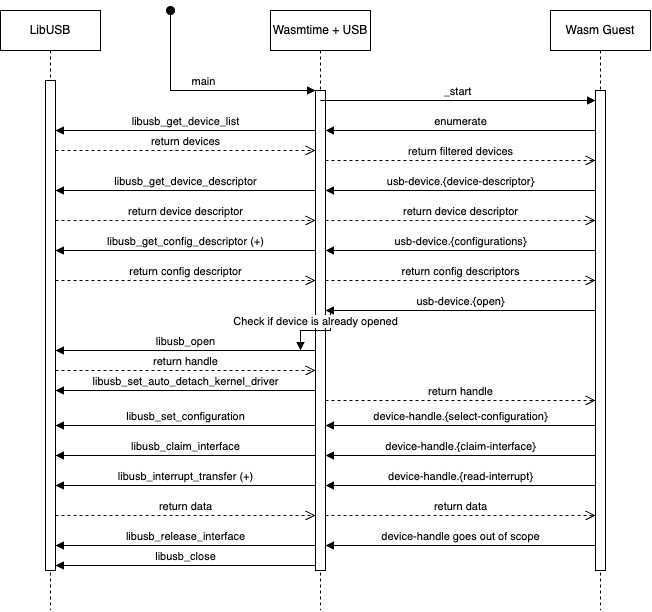
\includegraphics[width=0.8\textwidth]{images/sequentiediagram.png}
  \caption{Typical series of events sent between Wasm module - Wasmtime - libusb.}
  \label{fig:implementation_overview}
\end{figure}


\section{Runtime Implementation}
One of the requirements when proposing a new \acrshort{WASI} \acrshort{API} is to have multiple runtime implementations of that \acrshort{API}. This is required in order to advance to phase 3 of a proposal. The \acrshort{USB} \acrshort{WASI} proposal is still at phase 1. However, having a working implementation of the developing \acrshort{API} makes it easier to test out ideas and spot issues quickly. It also is useful to determine the viability of the \acrshort{API}. Therefore, a runtime implementation has been created before the proposal process had started.

When creating the \acrshort{PoC} implementation, a \acrshort{Wasm} runtime must be chosen which will be extended by the \acrshort{API}. There are numerous \acrshort{Wasm} runtimes available, such as Wasmtime \cite{wasmtime_website}, Wasmer \cite{wasmer} or WasmKit \cite{wasmkit}. Wasmtime was chosen for implementing the \acrshort{PoC}, as it has support for the Component Model and it is developed by the Bytecode Alliance \cite{bytecode_alliance}, the organization behind \acrshort{WASI}.

\subsection{Choosing the programming language}
The implementation is written in Rust \cite{rust_lang}, a system-level programming language which focuses on performance and safety. Rust's performance is similar to that of C, but its design eliminates entire classes of memory related bugs. Rust was an easy choice, as it has great support for \acrshort{Wasm} and \acrshort{WASI}, and Wasmtime is also written in it \cite{wasmtime_website}.

\subsection{Interfacing with libusb}
As told in Section \ref{section:libusb}, libusb will be used to communicate with operating-specific \acrshort{API}s to communicate with \acrshort{USB} devices. libusb is written in C \cite{LibUSB}. It is possible to interface with C in Rust. To make things easier, the Rusb \cite{rusb} package is used, which acts as a thin Rust wrapper around the libusb C \acrshort{API}.

\subsection{Interfacing with Wasmtime}
Wasmtime can be used in two ways: 
\begin{itemize}
\item Using the default Wasmtime runtime through the command line. A compiled \acrshort{Wasm} module can be passed as an argument:
\begin{minted}{bash}
$ wasmtime hello.wasm
Hello, world!
\end{minted}
\item Embedding the Wasmtime runtime in another app. The Bytecode Alliance provides packages in multiple languages, such as Rust or Go, to do this \cite{wasmtime_website}. This is the method used for creating the \acrshort{PoC} and is discussed further below.
\end{itemize}

The \acrshort{PoC} runtime embeds the Wasmtime runtime. The method of running is also similar: a compiled \acrshort{Wasm} module is passed as a command line argument.

Code snippet \ref{code:main} shows the main function of the runtime. First, the arguments are parsed, which contain the path to the component to run and identifiers of USB devices which are visible to components using the \acrshort{USB} \acrshort{API}. Next, the component gets instantiated (see code snippet \ref{code:start_component}) and an allowlist of devices is created. Finally, the component gets started.

The main function is annotated with \texttt{\#[tokio::main]}, meaning that the asynchronous Tokio runtime \cite{tokio} will be used. Tokio is an asynchronous runtime for Rust, and is not related to the Wasmtime runtime. The use of an asynchronous runtime is done for two reasons:
\begin{itemize}
\item The Wasmtime configuration in the runtime has enabled async support. At the time of writing, this isn't a really useful addition \cite{wasmtime_async_config}. However, this will become more useful once \acrshort{WASI} preview 3 lands, which will add proper async support to the \acrshort{WIT} language. Enabling async support now partially prepares for this upcoming feature.

\item The runtime receives updates when USB devices are connected and disconnected. This feature runs blocking functions which run on a separate thread. Tokio makes this easy to do.\\
\end{itemize}


\begin{code}
\begin{minted}[tabsize=4]{rust}
#[tokio::main]
async fn main() -> Result<()> {
	let parsed = UsbDemoAppParser::parse();
	let mut app = UsbDemoApp::new(parsed.component_path)?;

	let allowed_devices = if parsed.usb_use_denylist {
		AllowedUSBDevices::Denied(parsed.usb_devices)
	} else {
		AllowedUSBDevices::Allowed(parsed.usb_devices)
	};

	app.start(allowed_devices).await?
		.map_err(|_| anyhow!("Failed to run component."))
}
\end{minted}
\caption{The main function will start running the guest component.}
\label{code:main}
\end{code}

Code snippet \ref{code:start_component} shows how the passed in component will get instantiated. The \texttt{main} function first calls the \texttt{new} function. This function creates some necessary objects: 
\begin{itemize}
\item \texttt{Config}: The configuration used when creating a new \texttt{Engine}.
\item \texttt{Engine}: An engine manages and compiles \acrshort{Wasm} modules.
\item \texttt{Linker}: A linker is used to link components. Each component defines imports and exports. The linker is used to resolve these imports and exports, and throw errors if the required imports cannot be resolved.
\item \texttt{Component}: Used to represent a \acrshort{WASI} component.
\item \texttt{Store}: A Store is a collection of WebAssembly instances and host-defined state.
All WebAssembly instances and items will be attached to and refer to a Store. For example instances, functions, globals, and tables are all attached to a Store. Instances are created by instantiating a Module within a Store. \cite{wasmtime_store}
\end{itemize}

Next, the built-in components are added to the linker. \texttt{wasmtime\_wasi::add\_to\_linker\_async} adds all the standard Wasmtime components to the linker, such as \texttt{wasi:cli/stdout}. \texttt{Imports::add\_to\_linker} links the USB \acrshort{WIT} interface. Finally, the command component is loaded in and compiled.

The \texttt{start} function creates a new \texttt{Store} object. This object is associated with the earlier created engine, and contains the memory for an instance of \texttt{USBHostWasiView}. Finally, an instance of the guest component is created. We assume that the component is a \texttt{Command} (\ref{section:component_kinds}) and therefore exposes a \texttt{main} function. The \texttt{main} function, in \acrshort{WASI} terms also known as the \texttt{\_start} function, gets called.\\

\begin{code}
\begin{minted}[tabsize=4, breaklines]{rust}
struct UsbDemoApp {
	engine: Engine,
	linker: Linker<USBHostWasiView>,
	component: Component
}

impl UsbDemoApp {
	fn new(component: PathBuf) -> Result<Self> {
		let mut config = Config::default();
		config.wasm_component_model(true);
		config.async_support(true);

		let engine = Engine::new(&config)?;
		let mut linker = Linker::new(&engine);

		wasmtime_wasi::add_to_linker_async(&mut linker)?;
		Imports::add_to_linker(&mut linker, |view| view)?;
		
		let component = Component::from_file(&engine, component)?;

		Ok(Self {
			engine,
			linker,
			component
		})
	}

	async fn start(&mut self, allowed_devices: AllowedUSBDevices) -> anyhow::Result<Result<(), ()>> {
		let data = USBHostWasiView::new(allowed_devices)?;
		let mut store = Store::new(&self.engine, data);
	
		let (command, _) = Command::instantiate_async(&mut store, &self.component, &self.linker).await?;
	
		command.wasi_cli_run().call_run(store).await
	}
}
\end{minted} 
\caption{Code for extending the Wasmtime runtime.}
\label{code:start_component}
\end{code}

\subsection{Conforming to the \acrshort{WIT} interface}
The runtime must conform to the \acrshort{WIT} interface described in Section \ref{section:usb_proposal}. This part of the code \textit{receives} requests from guest components using the interface. The communication between the host and a component happens through the canonical ABI \cite{canonical_abi}. As discussed in Section \ref{section:thecomponentmodel}, bindings can be used to ease the translation from and to the canonical ABI format. Wasmtime offers the \texttt{bindgen} macro \cite{wasmtime_component_bindgen} to generate such bindings in Rust.

The usage of the \texttt{bindgen} macro is shown in code snippet \ref{code:wit_bindgen}.
This macro will generate Rust types and traits that represent their \acrshort{WIT} counterparts. The host must conform to all these traits. Otherwise, adding the \acrshort{USB} \acrshort{WIT} interface to the linker will be disallowed.

The \texttt{with} map shown in code snippet \ref{code:wit_bindgen} is used to point the \texttt{bindgen} tool to the Rust types we want to use to represent the \texttt{usb-device} and \texttt{device-handle} resources. The \texttt{bindgen} macro will use these types in the generated traits.\\

\newpage

\begin{code}
\begin{minted}[tabsize=4, breaklines]{rust}
pub mod bindings {
	wasmtime::component::bindgen!({
		world: "component:usb/imports",
		async: true,
		with: {
			"component:usb/usb/usb-device": crate::device::usbdevice::USBDevice,
			"component:usb/usb/device-handle": crate::device::devicehandle::DeviceHandle,
		},
		path: "../WIT/wit"
	});
}
\end{minted} 
\caption{Bindings are generated by using the Wasmtime \texttt{bindgen} macro.}
\label{code:wit_bindgen}
\end{code}

Code snippet \ref{code:conforming_example} shows an example usage of the generated bindings:
\begin{itemize}
\item \textbf{\texttt{USBHostWasiView}} is the type that implements the \acrshort{USB} \acrshort{WIT} interface. An instance of this type is passed to the linker to represent the \acrshort{USB} interface. The type checker verifies that \texttt{USBHostWasiView} conforms to all the required traits.
\item \textbf{\texttt{HostDeviceHandle}} is the trait generated by the bindings. It contains functions which \texttt{USBHostWasiView} needs to conform to.
\item \textbf{\texttt{Resource<DeviceHandle>}} is a reference to an \texttt{DeviceHandle} instance. 
\end{itemize}

\texttt{DeviceHandle} has a handle that is used to call libusb functions. In this example, the \texttt{claim\_interface} function will call the equivalent libusb function and return its result.\\

\newpage

\begin{code}
\begin{minted}[tabsize=4, breaklines]{rust}
#[async_trait]
impl HostDeviceHandle for USBHostWasiView {
	async fn claim_interface(&mut self, handle: Resource<DeviceHandle>, interface: u8) -> Result<Result<(), DeviceHandleError>> {
		let result = self.table()
			.get_mut(&handle)?
			.handle
			.claim_interface(interface)
			.map_err(|e| e.into());
	
		Ok(result)
	}
}

pub struct DeviceHandle {
	pub handle: rusb::DeviceHandle<rusb::Context>
}
\end{minted} 
\caption{An example of using generated bindings. An implementation for \texttt{claim-interface} is provided.}
\label{code:conforming_example}
\end{code}

\subsection{Conforming to constraints}
Section \ref{section:capability_based_security} and \ref{section:usage_in_multiple_components} mention important constraints regarding the correct implementation of the API. The implementation conforms to the following constraints.

\paragraph{Capability-based security}
As seen in code snippet \ref{code:main}, an allowlist gets created, containing a series of device IDs. A device is identified by the pair \texttt{vendor\_id:product\_id}. These can be passed in as arguments when running the program. An optional flag \texttt{--usb-use-denylist} can be given so the program uses a denylist instead of an allowlist.

\begin{verbatim}
cargo run -- --usb-devices 18d1:9400,18d1:9401 guest-component.wasm
\end{verbatim}

Table \ref{table:allowlist} shows the four configurations that are possible. The functions \texttt{usb-device.\{enumerate\}} and \texttt{events.\{update\}} will use this configuration to filter out devices that should not be visible.

\begin{table}[h!]
\centering
\begin{tabular}{|c|c|c|}
\hline
& \textbf{Allowlist} & \textbf{Denylist} \\
\hline
\textbf{Devices Specified} & specified devices allowed & all but specified allowed \\
\hline
\textbf{No devices specified} & no device allowed & all allowed \\
\hline
\end{tabular}
\caption{Device access control options.}
\label{table:allowlist}
\end{table}

\paragraph{Usage in multiple components} Exclusive access to devices is guaranteed by keeping track of the device handles. Only one \texttt{device-handle} instance may exist for each \acrshort{USB} device. \texttt{USBHostWastView} stores a set of device addresses for devices with an active \texttt{device-handle}. It does not keep track of which component uses which device. When a \texttt{device-handle} gets dropped, the device address is removed from the set and becomes available again. When a component tries opening an already-opened device, an error will be thrown. 

\subsection{Platform limitations}
\label{section:platform_limitations}
The current host implementation works on Linux, macOS and Windows. However, some features work slightly different on some platforms:

\begin{itemize}
\item macOS: 
\begin{itemize}
\item Using devices for which the kernel provides drivers is disallowed, unless the program has elevated privileges, for example using \texttt{sudo} \cite{libusb_macos_limitations}.
\end{itemize}

\item Windows:
\begin{itemize}
\item libusb hotplug support is currently missing for Windows. This feature is used in the implementation to get device connection events. Recent activity shows that this might come soon \cite{libusb_hotplug_support}.
\item HID keyboards and mice cannot be accessed using the native HID driver as Windows reserves exclusive access to them \cite{libusb_windows_limitations}. 
\end{itemize}
\end{itemize}

\section{Usage in guest components}
This section demonstrates how a \acrshort{WASI} component can use the \acrshort{USB} \acrshort{API}. Parts of the code used for the program in Section \ref{section:functional_evaluation} will be explained.

\subsection{Defining a \acrshort{WIT} interface}
The guest component is required to also provide a \acrshort{WIT} interface, shown in code snippet \ref{code:guest_world}. The interface contains a single \texttt{root} world, describing the imports and exports required by the component. The guest component explained here is a Command component (\ref{section:component_kinds}), and therefore does not need to provide any exports. In order to use the \acrshort{USB} \acrshort{API}, it will import all the interfaces of the \acrshort{USB} component.\\

\begin{code}
\begin{lstlisting}[breaklines, language=wit, tabsize=4]
package component:usb-component-wasi-stadia;

world root {
	import component:usb/types@0.2.0;
	import component:usb/usb@0.2.0;
	import component:usb/events@0.2.0;
	import component:usb/descriptors@0.2.0;
}
\end{lstlisting}
\caption{The \acrshort{WIT} world for the guest component.}
\label{code:guest_world}
\end{code}

\subsection{Creating a \acrshort{Wasm} module}
The code written for the guest component must be compiled to a .wasm file. Doing this can be time consuming, as multiple steps are required:

\begin{enumerate}
\item Create bindings.
\item Build a \acrshort{Wasm} module.
\item Create a new \acrshort{WASI} component and apply the adapter for \acrshort{WASI} preview 2.
\end{enumerate}

In order to ease this process, the Cargo-component tool \cite{cargo_component} was created. By running
\begin{verbatim}
cargo component build
\end{verbatim}
the tool will interpret the \acrshort{WIT} interface, generate bindings for Rust code, and produce a compiled \acrshort{Wasm} module. The guest component makes use of this tool to produce a \acrshort{Wasm} module with ease.

\subsection{Calling the \acrshort{USB} \acrshort{API}}
Now that the \acrshort{WIT} interface is defined and bindings are created, calling the USB API is straightforward. Code snippet \ref{code:calling_usb_api} shows the \texttt{main} function of the guest component. This function will start listening to connection events, and calls the \texttt{component:usb/events{update}} function to get these events. Next, it will match the event using the \texttt{component:usb/events{device-connection-event}} variant. As can be seen in the code snippet, these \acrshort{WASI} types are translated to Rust types and can be imported into the file. Then, they can be used like regular Rust code. \\

\begin{code}
\begin{minted}[tabsize=4, breaklines]{rust}
use crate::bindings::component::usb::{
	usb::UsbDevice, 
	events::DeviceConnectionEvent
};

#[tokio::main(flavor = "current_thread")]
async fn main() -> anyhow::Result<()> {
	loop {
		match update() {
			DeviceConnectionEvent::Pending => sleep(Duration::from_secs(1)).await,
			DeviceConnectionEvent::Connected(device) if device.is_stadia_device() => {
				// Found stadia controller
				... // Handle
			},
			DeviceConnectionEvent::Disconnected(device) if device.is_stadia_device() => {
				// Stadia controller is removed
				... // Handle
			},
			_ => continue
		}
	}
}
\end{minted} 
\caption{The \acrshort{WIT} world for the guest component.}
\label{code:calling_usb_api}
\end{code}

